% DO NOT COMPILE THIS FILE DIRECTLY!
% This is included by the other .tex files.

\begin{frame}
\titlepage
\end{frame}

\begin{frame}
  \frametitle{The aim of this presentation}
  \begin{itemize}
     \item A small update of what has happened around MISP's development over the past few months
     \item Our initial scope
     \item Why is {\bf contextualisation} important?
     \item What options do we have in MISP?
     \item How can we {\bf leverage} this in the end?
  \end{itemize}
\end{frame}

\begin{frame}
  \frametitle{MISP's evolution since the last MUG}
  \begin{itemize}
    \item Since the last MUG (05/12/2019) we've had:
    \begin{itemize}
        \item 8 releases
        \item 2196 commits
        \item 85 contributors contributing to the core software and its components
    \end{itemize}
    \item COVID-19 didn't negatively impact the progress made all that much
  \end{itemize}
\end{frame}

\begin{frame}
  \frametitle{So what were the main changes?}
  \begin{itemize}
     \item Loads of bug fixes
     \item A host of improvements to how MISP functions
     \item Security fixes, including several CVEs (keep your MISP up to date!)
     \item Generally loads of internal improvements (in large part thanks to Jakub Onderka)
     \item Massively expanding context libraries
     \item Several major features (let's talk about these)
  \end{itemize}
\end{frame}

\begin{frame}
\frametitle{Timelining in MISP}
\begin{itemize}
	\item The goal was to capture activity timelines
        \item All attributes and objects can have first-seen/last-seen data       
\end{itemize}
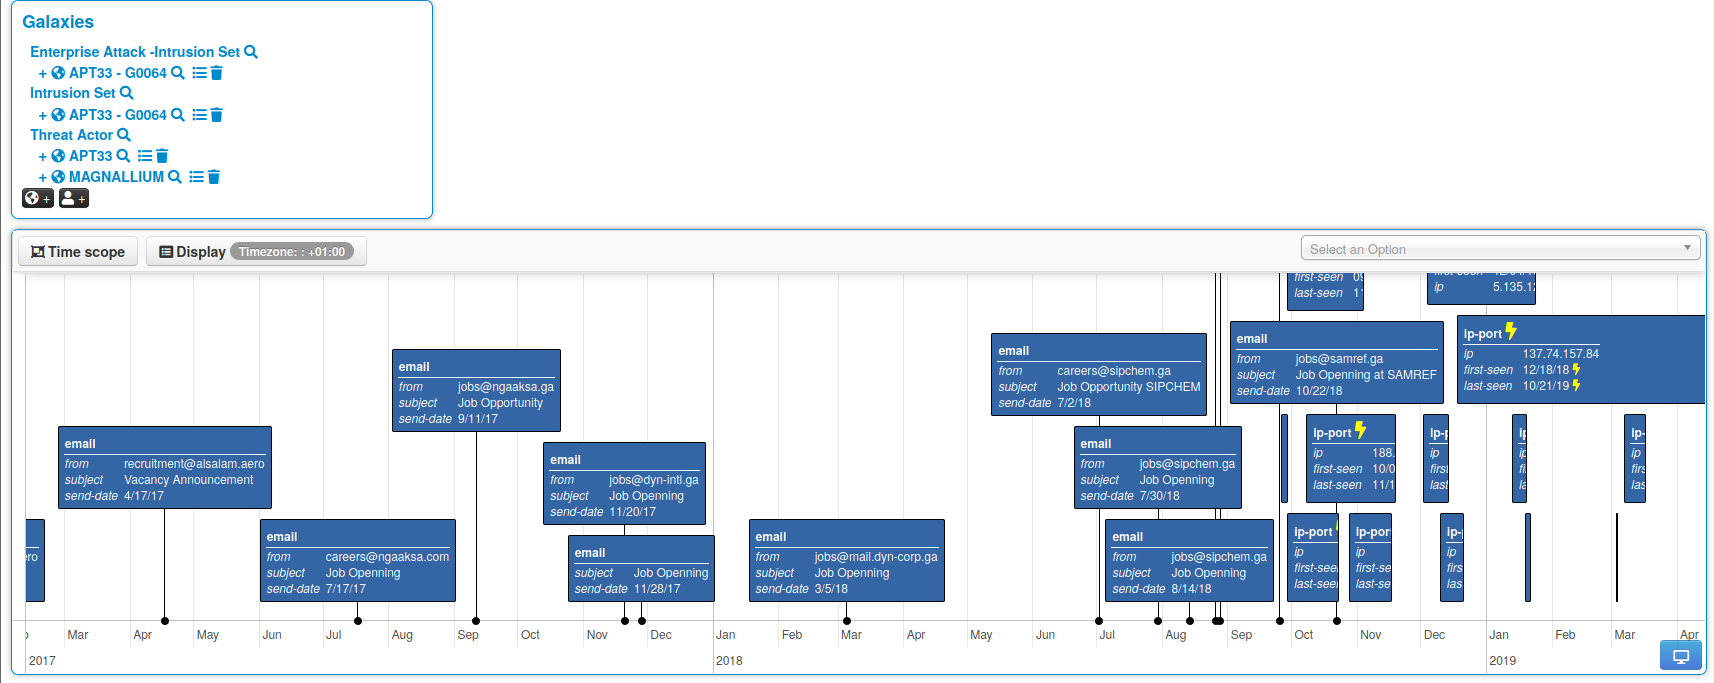
\includegraphics[scale=0.25]{images/timeline.png}
\end{frame}

\begin{frame}
\frametitle{Timelining in MISP}
\begin{itemize}
	\item Why is this interesting?
        \item {\bf IoC lifecycle management} is one of the biggest challenges we face
        \item Timeline information allows us to better {\bf express a story}, rather than {\bf share dumps of IoCs}
        \item {\bf Time-based correlation} of certain actions helps us understand an incident
\end{itemize}
\end{frame}

\begin{frame}
\frametitle{Dashboarding}
\begin{itemize}
	\item Outcome of our personal initiatives to track the COVID-19 spread
        \item New built-in {\bf dashboarding system} directly available in MISP
        \item Dashboard widgets are modular and {\bf easy to build}
        \item Create widgets that are {\bf ACL aware}
        \item The COVID-19 MISP community turned out to be a massive success
        \item COVID-19 use-cases are just an example though (admin widgets, trend widgets, etc)
\end{itemize}
\end{frame}

\begin{frame}
\frametitle{Dashboarding}
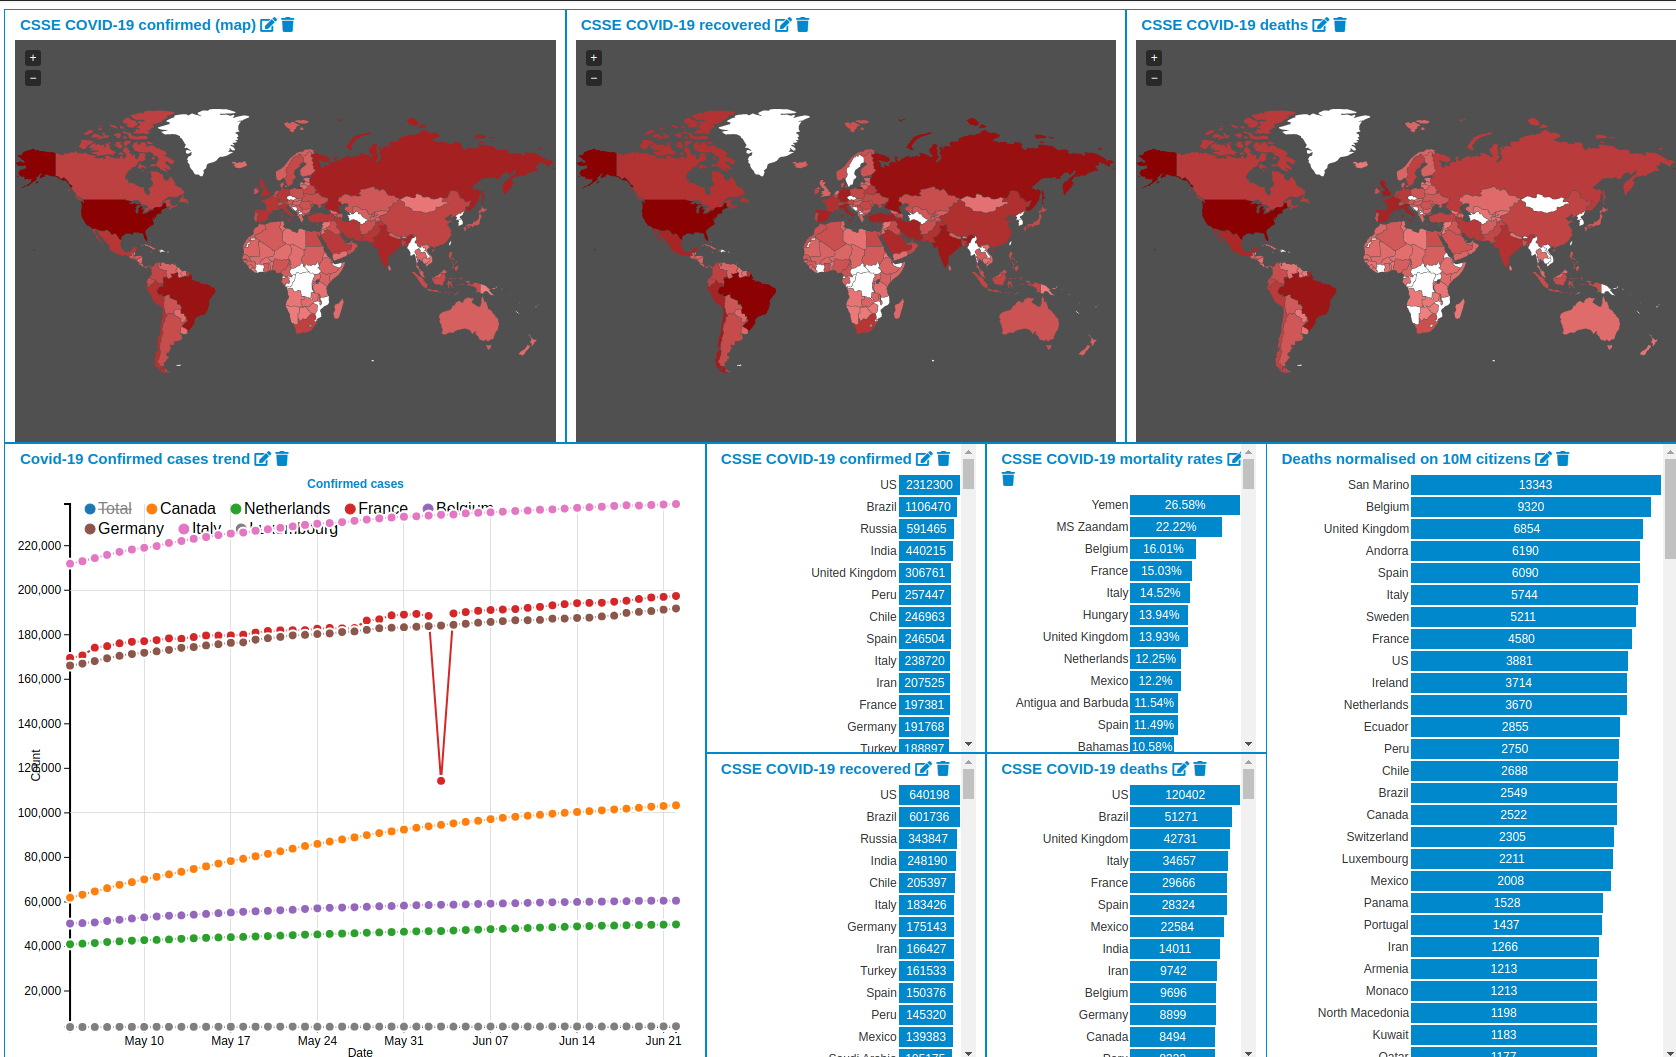
\includegraphics[scale=0.25]{images/dashboard.png}
\end{frame}


\begin{frame}
\frametitle{Decaying indicators v2}
\begin{itemize}
	\item {\bf User settings} are now taken into account when crafting queries
        \item {\bf Tool specific} user accounts can be pre-configured with decaying settings
        \item {\bf Taxonomy} numerical values can be re-mapped to fit internal needs
        \item {\bf Sightings} factor into the decay scores
\end{itemize}
\end{frame}

\begin{frame}
\frametitle{Massive rewrite of PyMISP}
\begin{itemize}
	\item Python 3.6+ is a minimum since the modern PyMISP rework
        \item Use of {\bf objects} with a {\bf long list of helpers} allows for easy creation/modification of MISP data
        \item PyMISP's {\bf CI testing} suite has grown massively, allowing us to catch more and more issues as we commit changes
        \item Automated testing {\bf including synchronising} several MISP instances
\end{itemize}
\end{frame}

\begin{frame}
\frametitle{Community management improvements}
\begin{itemize}
	\item {\bf User configurations} allow users to manage different aspects of how they use MISP (for example {\bf alerting rules})
        \item {\bf Community listings} directly in MISP help new users find the right points of contact (perhaps something for NATO to consider?)
        \item {\bf E-mail based OTP} - Implemented by NCIA's very own Loïc Fortemps
\end{itemize}
\end{frame}

\begin{frame}
\frametitle{Integrations}
\begin{itemize}
	\item Long list of {\bf integrations}, both via our export system and module systems and by other tools integrating with MISP
        \item Continuous iterations of our connectors using other formats (a massive STIX 2 rework has just dropped)
        \item Integrations with analysis tools, such as with Maltego (thanks to Christophe Vandeplas)
        \item Tighter integration with other OSS frameworks we develop in-house (AIL, D4)
        \item Mapping of libraries to taxonomies/galaxies/object templates
        \item ATT\&CK like matrices from other domains (disinformation via AMITT, various sectorial groups)
\end{itemize}
\end{frame}

\begin{frame}
\frametitle{So that's where we are now}
\begin{itemize}
	\item Let's have a brief look at what is on our immediate and long-term roadmaps
        \item For the long-term ones, priorities shift rapidly
\end{itemize}
\end{frame}


\begin{frame}
\frametitle{MISP galaxy 2.0}
\begin{itemize}
	\item MISP galaxies will be fully managed via MISP directly
        \item Create, modify, {\bf share your custom galaxies} with the usual sync / ACL mechanisms
        \item Fork and {\bf provide your own perspective} to already existing knowledge-base items
        \item Build {\bf relationships between galaxy clusters} (Threat actor A uses Tool B and targets Sector C)
\end{itemize}
\end{frame}

\begin{frame}
\frametitle{Reports}
\begin{itemize}
	\item Create {\bf markdown reports} and share them along with your events
        \item Structured information is great for automation, but sometimes plain prose helps telling a story
\end{itemize}
\end{frame}

\begin{frame}
\frametitle{Community management at scale}
\begin{itemize}
	\item Cerebrate is a new OSS frameworks that we're building
        \item Manage organisation, sharing group, encryption key data for communities
        \item Instrument MISP instances and the interconnectivity between them via Cerebrate
        \item Introduce information signing by validating signatures / ownership via trusted Cerebrate nodes
\end{itemize}
\end{frame}

\begin{frame}
\frametitle{Rework of the MISP internals}
\begin{itemize}
	\item We are planning on moving MISP to a {\bf more modern stack} (cake4/bs4)
        \item Cerebrate also acts as a {\bf test-bed} for this move and relies on MISP internals that have already been ported
        \item We have been silently {\bf reworking a lot of the internals} of MISP to make the migration possible (UI generator systems for example)
\end{itemize}
\end{frame}

\begin{frame}
  \frametitle{To sum it all up...}
  \begin{itemize}
     \item Many interesting things are happening
     \item We are following {\bf several routes} of development (internal improvements, contextualisation, integrations, operational improvements, community building)
     \item We have more ideas than can be implemented with days only having 24 hours, there are {\bf many ways to get involved}
     \item Prioritisation is hard. {\bf Let us know what you think we should focus on}!
  \end{itemize}
\end{frame}

\begin{frame}
  \frametitle{Get in touch if you have any questions}
  \begin{itemize}
    \item Contact CIRCL
    \begin{itemize}
      \item info@circl.lu
      \item \url{https://twitter.com/circl_lu}
      \item \url{https://www.circl.lu/}
    \end{itemize}
    \item Contact MISPProject 
    \begin{itemize}
      \item \url{https://github.com/MISP}
      \item \url{https://gitter.im/MISP/MISP}
      \item \url{https://twitter.com/MISPProject}
    \end{itemize}
    \item Join the COVID-19 MISP community
    \begin{itemize}
      \item \url{https://covid-19.iglocska.eu}
    \end{itemize}
  \end{itemize}
\end{frame}
